\let\negmedspace\undefined
\let\negthickspace\undefined
\documentclass[journal]{IEEEtran}
\usepackage[a5paper, margin=10mm, onecolumn]{geometry}
%\usepackage{lmodern} % Ensure lmodern is loaded for pdflatex
\usepackage{tfrupee} % Include tfrupee package

\setlength{\headheight}{1cm} % Set the height of the header box
\setlength{\headsep}{0mm}     % Set the distance between the header box and the top of the text

\usepackage{gvv-book}
\usepackage{gvv}
\usepackage{cite}
\usepackage{amsmath,amssymb,amsfonts,amsthm}
\usepackage{algorithmic}
\usepackage{graphicx}
\usepackage{textcomp}
\usepackage{xcolor}
\usepackage{txfonts}
\usepackage{listings}
\usepackage{enumitem}
\usepackage{mathtools}
\usepackage{gensymb}
\usepackage{comment}
\usepackage[breaklinks=true]{hyperref}
\usepackage{tkz-euclide} 
\usepackage{listings}
% \usepackage{gvv}                                        
\def\inputGnumericTable{}                                 
\usepackage[latin1]{inputenc}                                
\usepackage{color}                                            
\usepackage{array}                                            
\usepackage{longtable}                                       
\usepackage{calc}                                             
\usepackage{multirow}                                         
\usepackage{hhline}                                           
\usepackage{ifthen}                                           
\usepackage{lscape}
\begin{document}

\bibliographystyle{IEEEtran}
\vspace{3cm}

\title{5.2.36}
\author{EE25BTECH11033 - Kavin}
% \maketitle
% \newpage
% \bigskip
{\let\newpage\relax\maketitle}

\renewcommand{\thefigure}{\theenumi}
\renewcommand{\thetable}{\theenumi}
\setlength{\intextsep}{10pt} % Space between text and floats
\textbf{Question}:\\
Solve the following system of linear equations.
\begin{align*}
    3x-5y-4=0
\end{align*}
\begin{align*}
    9x=2y+7
\end{align*}
\bigskip


\textbf{Solution}:\\
The equation of line $L_1$ is,
\begin{align}
    \myvec{3 & -5}\vec{x} = 4
\end{align}
The equation of line $L_2$ is,
\begin{align}
    \myvec{9 & -2}\vec{x} = 7
\end{align}
On putting the equations in a matrix, we will get
\begin{align}
    \implies \myvec{3 & -5\\9 & -2}\vec{x} = \myvec{4\\7}
\end{align}
So the augmented matrix is,
\begin{align}
    \augvec{2}{1}{3 & -5 & 4\\9 & -2 & 7}
\end{align}
\begin{align}
    R_2\rightarrow R_2-3R_1\implies\augvec{2}{1}{3 & -5 & 4\\0 & 13 & -5}
\end{align}
\begin{align}
    R_2\rightarrow \frac{1}{13}R_2\implies\augvec{2}{1}{3 & -5 & 4\\0 & 1 & -5/13}
\end{align}
\begin{align}
    R_1\rightarrow R_1+5R_2\implies\augvec{2}{1}{3 & 0 & 27/13\\0 & 1 & -5/13}
\end{align}
\begin{align}
    R_1\rightarrow \frac{1}{3}R_1\implies\augvec{2}{1}{1 & 0 & 9/13\\0 & 1 & -5/13}
\end{align}
\begin{align}
    \implies\vec{x} =\myvec{x\\y}\equiv \myvec{9/13\\-5/13}
\end{align}
Therefore the two lines will intersect at \myvec{9/13\\-5/13}.\\
\bigskip

\begin{figure}[H]
\begin{center}
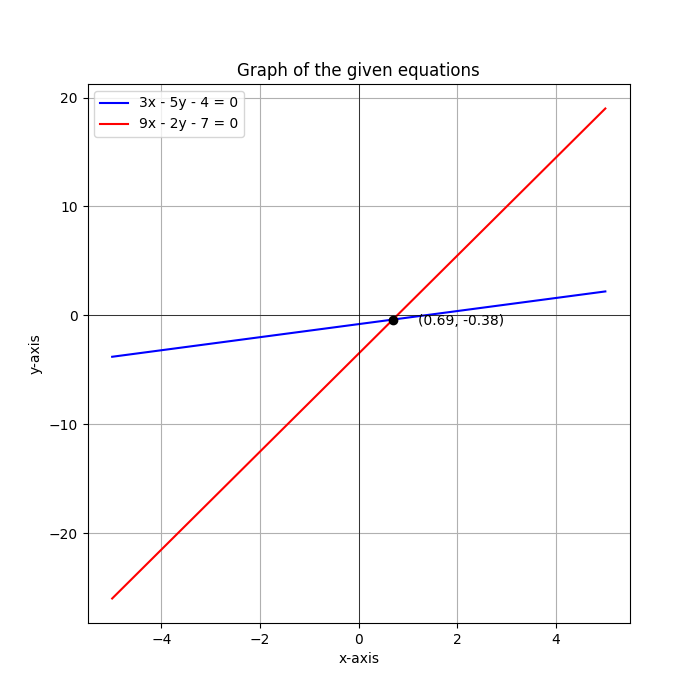
\includegraphics[width=0.8\columnwidth]{figs/fig.png}
\end{center}
\label{fig:Fig1}
\end{figure}
\end{document}


